% !TEX TS-program = pdflatex
% !TEX encoding = UTF-8 Unicode

% This is a simple template for a LaTeX document using the "article" class.
% See "book", "report", "letter" for other types of document.

%tells you if you use obsolote packages
%\RequirePackage[l2tabu,orthodox]{nag}

\documentclass[]{article}

\usepackage[utf8]{inputenc} % set input encoding (not needed with XeLaTeX)

%%% PAGE DIMENSIONS
\usepackage{geometry} % to change the page dimensions
\geometry{a4paper} % or letterpaper (US) or a5paper or....
% \geometry{margin=2in} % for example, change the margins to 2 inches all round
% \geometry{landscape} % set up the page for landscape
%   read geometry.pdf for detailed page layout information

\usepackage{graphicx} % support the \includegraphics command and options

% \usepackage[parfill]{parskip} % Activate to begin paragraphs with an empty line rather than an indent

%%% PACKAGES
\usepackage{booktabs} % for much better looking tables
\usepackage{array} % for better arrays (eg matrices) in maths
\usepackage{paralist} % very flexible & customisable lists (eg. enumerate/itemize, etc.)
\usepackage{verbatim} % adds environment for commenting out blocks of text & for better verbatim
\usepackage{subfig} % make it possible to include more than one captioned figure/table in a single float
\usepackage{microtype} %makes awesome kerning and punctuation come half way out the edge of the text
\usepackage{listings} %for code listings
\usepackage{color} %for colored syntax highligting
\usepackage{rotating}
\usepackage{pdflscape}
\usepackage[]{algorithm2e}

%%% Code listing
\definecolor{mygreen}{rgb}{0,0.6,0}
\definecolor{mygray}{rgb}{0.5,0.5,0.5}
\definecolor{mymauve}{rgb}{0.58,0,0.82}
\lstset{breaklines=true,
basicstyle=\footnotesize\ttfamily,
commentstyle=\color{mygreen},
keywordstyle=\color{blue},
numberstyle=\tiny\color{mygray},
tabsize=2,
frame=tb,
aboveskip=5mm,
belowskip=0mm,
breaklines=true,
breakatwhitespace=true
}

% to include a file as a listing: \lstinputlisting{intio.c}
% inline listing: \begin{lstlisting}[frame=single]

%%% HEADERS & FOOTERS
\usepackage{fancyhdr} % This should be set AFTER setting up the page geometry
\pagestyle{fancy} % options: empty , plain , fancy
\renewcommand{\headrulewidth}{0pt} % customise the layout...
\lhead{}\chead{}\rhead{}
\lfoot{}\cfoot{\thepage}\rfoot{}

%%% ToC (table of contents) APPEARANCE
\usepackage[nottoc,notlof,notlot]{tocbibind} % Put the bibliography in the ToC
\usepackage[titles,subfigure]{tocloft} % Alter the style of the Table of Contents
%\renewcommand{\cftsecfont}{\rmfamily\mdseries\upshape}
%\renewcommand{\cftsecpagefont}{\rmfamily\mdseries\upshape} % No bold!
\usepackage{hyperref} % use hyperlinked ToC
\hypersetup{colorlinks=true, linkcolor=black, citecolor=black, filecolor=black, urlcolor=black}

%%%-------------------------------------------------------------------


\title{Digital System Design Report}
\author{Oskar Weigl - ow610\\ and \\ Ryan Savitski - rs510}
%\date{} % Activate to display a given date or no date (if empty),
         % otherwise the current date is printed 

\begin{document}
\maketitle

%\renewcommand{\abstractname}{Summary}
\begin{abstract}
	Write the abstract here
\end{abstract}

\tableofcontents
\clearpage



\section{Floating Point Hardware} % (fold)
\label{sec:floating_point_hardware}


\begin{table}[tbp]
	\caption{Hardware setup for the floating point performance measurements.}
	\label{tab:fp_hw_setup}
	\begin{center}
		\begin{tabular}{r|l}
		\hline

		\hline
			\textbf{Processor Type} 	& Nios II Standard \\
		\hline
			\textbf{Instruction Cache}	& 2 kB \\
		\hline
			\textbf{Data Cache}			& none \\
		\hline
			\textbf{Clock Speed}		& 50 MHz \\
		\hline

		\hline
		\end{tabular}
	\end{center}
\end{table}


\begin{table}[tbp]
	\caption{Performance comparison of software determinant calculation for various hardware configurations and matrix sizes. The algorithm used is based on LU decomposition and the hardware is set up as shown in Table~\ref{tab:fp_hw_setup}. Entries are time in milliseconds per matrix.}
	\label{tab:sw_perf}
	\begin{center}
		\begin{tabular}{r|ccccc}
		\hline

		\hline
			& \textbf{3x3}	& \textbf{6x6}	& \textbf{8x8}	& \textbf{10x10}	& \textbf{20x20} \\ 
		\hline
			\textbf{No hardware multipliers}
			& 0.940			& 6.6			& 15.3			& 30.1				& 231.75 \\
		\hline
			\textbf{Embedded multipliers}
			& 0.470			& 3.15			& 8.0			& 14.4				& 115.5 \\
		\hline
			\textbf{Custom floating-point instructions}
			& 0.122			& 0.468			& 0.984			& 1.450				& 7.8 \\
		\hline

		\hline
		\end{tabular}
	\end{center}
\end{table}

the matrix algorithm is constant for each size: 49 KB


We use a modified version of the Doolittle Algorithm for LU decomposition to compute the determinant. This algorithm is discussed in more detail in Section~\ref{sub:theory}.


% section floating_point_hardware (end)





\section{Determinant Calculation Hardware Accelerator} % (fold)
\label{sec:determinant_calculation_hardware_accelerator}

PUT INTRODUCTION HERE!

IEEE 754 single precision \cite{ieee754}.

\subsection{Theory} % (fold)
\label{sub:theory}

\begin{algorithm}[htbp]
	\SetAlgoLined

	\KwData{N x N matrix: A}
	\KwResult{Determinant}

	\For{k = 1 \KwTo N - 1}{
		
		\While{$a_{k,k} = 0$}{
			rotate rows $k$ to $N$\;
			\If{number of rotations = k}{
				determinant $\leftarrow 0$ \\
				return;
			}
		}

		\For{i = k + 1 \KwTo N}{
			$a_{i,k} \leftarrow a_{i,k}/a_{k,k}$
		}

		\For{j = k+1 \KwTo N}{
			\For{i = k+1 \KwTo N}{
				$a_{i,j} \leftarrow a_{i,j} - a_{i,k} \times a_{k,j}$
			}
		}
	}

	determinant $\leftarrow \prod_{k=1}^N a_{k,k}$
	\bigskip

	\caption{The Doolittle Algorithm for computing the LU decomposition of a matrix, as found in \cite{LUgen}, but modified to compute the determinant, and include pivoting.}
	\label{alg:doolittle}
\end{algorithm}

This hardware module uses a modified version of the Doolittle Algorithm to compute the determinant of a matrix.
We implement a 

% subsection theory (end)

\subsection{Interface Overview} % (fold)
\label{sub:interface_overview}


% subsection interface_overview (end)


\subsection{Operation} % (fold)
\label{sub:det_operation}


% subsection operation (end)


\subsection{Implementation Details} % (fold)
\label{sub:implementation_details}


% subsection implementation_details (end)


\subsection{Performance} % (fold)
\label{sub:performance}


% subsection performance (end)


\subsection{Scalability} % (fold)
\label{sub:scalability}


% subsection scalability (end)




\begin{table}[htbp]
	\caption{Resource Utilisation of the Determinant module. Note that two fp\_mul units are used.}
	\label{tab:resource_util_det}
	\begin{center}
		\begin{tabular}{l|ccccc}
		\hline

		\hline
											& \textbf{Entire Module} 	& \textbf{fp\_div} 		& \textbf{fp\_mul}	& \textbf{fp\_sub} 	& \textbf{matrixram} \\
		\hline
			\textbf{Logic Cells} 			& 5978						& 404 					& 264 				& 827 				& 0 \\
		\hline
			\textbf{Dedicated Registers}	& 3663						& 291 					& 208 				& 426				& 0 \\
		\hline
			\textbf{M9K Memory Blocks}		& 11						& 6 					& 0 				& 1 				& 4 \\
		\hline
			\textbf{Multiplier Elements}	& 31						& 16 					& 7 				& 0					& 0 \\
		\hline

		\hline
		\end{tabular}
	\end{center}
\end{table}

\begin{figure}[htbp]
	\begin{center}
		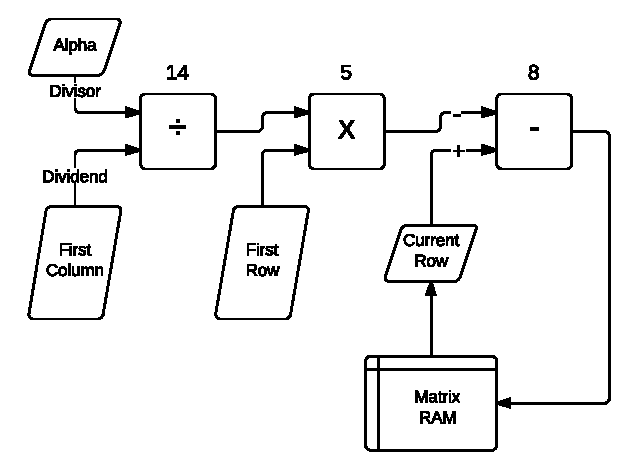
\includegraphics[width = 0.8\textwidth]{DeterminantPipeline.pdf}
	\end{center}
	\caption{Block diagram of the hardware implementation of the Doolittle Algorithm. The number above the arithmetic blocks indicate latency.}
	\label{fig:det_block}
\end{figure}

\begin{figure}[htbp]
	\begin{center}
		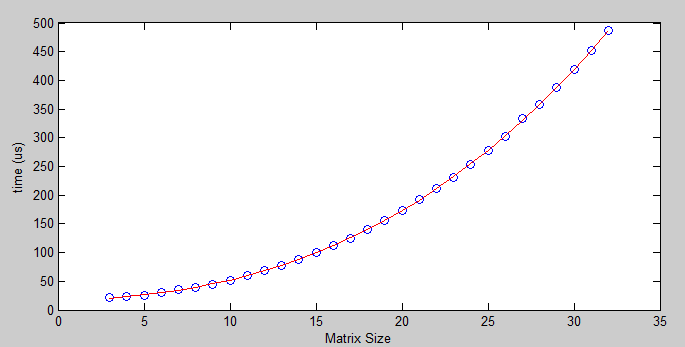
\includegraphics[width = \textwidth]{detcubicresult.PNG}
	\end{center}
	\caption{Benchmark results of the determinant hardware. Plotted in blue are the data points, and shown in red is a cubic regression, detailed in Table~\ref{tab:polyfit_coeffs}.}
	\label{fig:det_bench_results}
\end{figure}

\begin{table}[htbp]
	\caption{The result of the cubic regression shown in Figure~\ref{fig:det_bench_results}.}
	\label{tab:polyfit_coeffs}
	\begin{center}
		\begin{tabular}{l|cccc}
		\hline

		\hline
			& \textbf{$N^3$} & \textbf{$N^2$} & \textbf{$N$} & \textbf{$1$}\\
		\hline
			\textbf{Time} (ns)
			& 6.49 	& 236	& 490	& 17100 \\
		\hline
			\textbf{Time} (cycles)
			& 0.324 & 11.8 	& 24.5 	& 855 \\

		\hline
		\end{tabular}
	\end{center}
\end{table}


reffering to Algorithm~\ref{alg:doolittle}, we can identify the expected growth of different parts of the algorithm.

\begin{table}[htbp]
	\caption{Expected complexity of various operations in LU decomposition. Note that element multiplication and subtraction are pipelined and do not add.}
	\label{tab:expected_complexity}
	\begin{center}
		\begin{tabular}{l|c}
		\hline

		\hline
			\textbf{Element multiplication} 	& $N^3/2$ \\
		\hline
			\textbf{Element subtraction} 		& $N^3/2$ \\
		\hline
			\textbf{Matrix memory copy} 		& $N^2$ \\
		\hline
			\textbf{Pipeline flushes} 			& $N$ \\
		\hline
			\textbf{Division latency} 			& $N$ \\
		\hline
			\textbf{Diagonal multiplication} 	& $N$ \\
		\hline
			\textbf{Interrupt latency}			& 1 \\
		\hline
		
		\hline
		\end{tabular}
	\end{center}
\end{table}


% section determinant_calculation_hardware_accelerator (end)


\clearpage


\section{Notch Filter} % (fold)
\label{sec:notch_filter}

The Notch Filter module is a memory mapped hardware accelerator for the purpose of filtering a 16 bit signed input. It implements a 2nd order notch filter tuned to to remove any spectral components at 1 kHz.
The module is capable of Direct Memory Access, includes optimisations for efficient access to the SDRAM, and uses a buffering and Clock Domain Crossing strategy, to maximise performance.

\subsection{Filter Design} % (fold)
\label{sub:filter_design}

The chosen filter type is a 2nd order IIR filter. This filter order is the minimum required to generate the complex pole and zero pairs required to implement a notch filter. In fact, no higher order is needed, as the noise is a pure sinusoid, so the width of the stop-band can be very small, and as such, no additional zeroes are required.

The filter is designed by simply placing a complex zero on the unit circle corresponding to the 1 KHz null we wish to create. To cancel the effect of this zero for other frequencies, we place a complex pole very close to it on the inside of the unit circle. The bandwidth of the filter is tuned by moving the complex pole radially.

In our case, we elect to place the pole such that the bandwidth of rejection is about 25Hz. This is is chosen as a good trade-off for several reasons. Firstly, placing the pole at this location makes the filter robust to coefficient quantisation, as discussed in Section~\ref{sub:quantization}.
More importantly, this bandwidth is narrow enough to not affect the music, but wide enough to quickly suppress the overlaid sinusoid at the beginning of the sample.
The magnitude response of the resulting filter can been seen in Figure~\ref{fig:matlabmagnitudelog}.

Several different types of filter topologies are considered. Firstly, it is clear that as a 2nd order IIR filter meets the specification, it would be rather inappropriate to implement the same filter as an FIR filter. To get the same sharp transition band using an FIR filter, we would have to use over 10,000 taps.
This metric is generated using MATLAB's Parks-McClellan optimal equiripple FIR order estimator; the MATLAB command and result can be seen in Figure~\ref{fig:firpmord}.

\begin{figure}[bp]
	\begin{center}
		\begin{lstlisting}[language = Matlab]
beethmax = max(abs(fft(beeth5_noise)));
firpmord([987.5 999 1001 1012.5], [1 0 1], [0.01 10/beethmax 0.01], 44100)
ans = 13410
		\end{lstlisting}
	\end{center}
	\caption{MATLAB command to estimate the order of FIR filter required for the notch filter specification.}
	\label{fig:firpmord}
\end{figure}

\begin{figure}[htbp]
	\begin{center}
		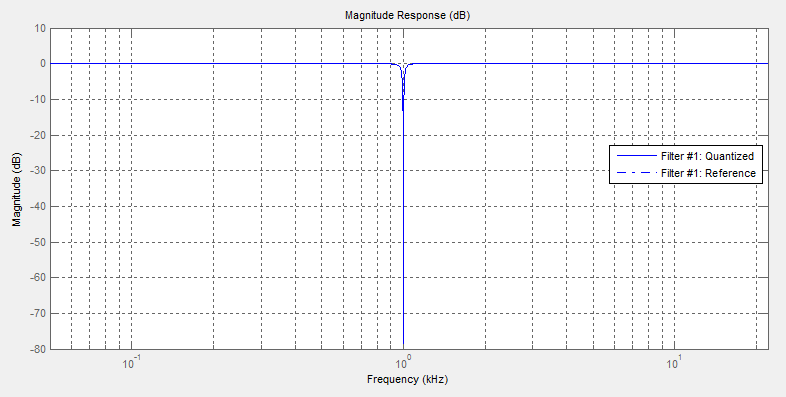
\includegraphics[width = \textwidth]{matlabmagnitudelog.PNG}
	\end{center}
	\caption{Magnitude response of both the full (double) precision and the quantised filter. The gain is negative infinity dB at 1 kHz.}
	\label{fig:matlabmagnitudelog}
\end{figure}

\begin{figure}[htbp]
	\begin{center}
		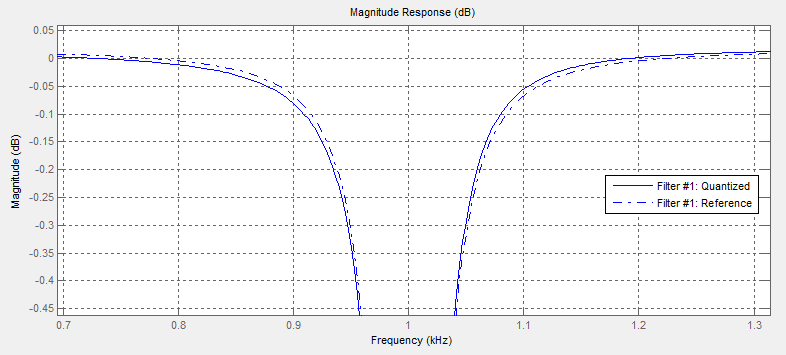
\includegraphics[width = \textwidth]{matlabmagnitude2.PNG}
	\end{center}
	\caption{Magnitude response of both the full (double) precision and the quantised filter. The quantised and reference filters differ with less than 0.02dB in the passband.}
	\label{fig:matlabmagnitudezoom}
\end{figure}

% subsection filter_design (end)

\subsection{Filter Topology} % (fold)
\label{sub:filter_topology}

\begin{figure}[btp]
	\begin{center}
		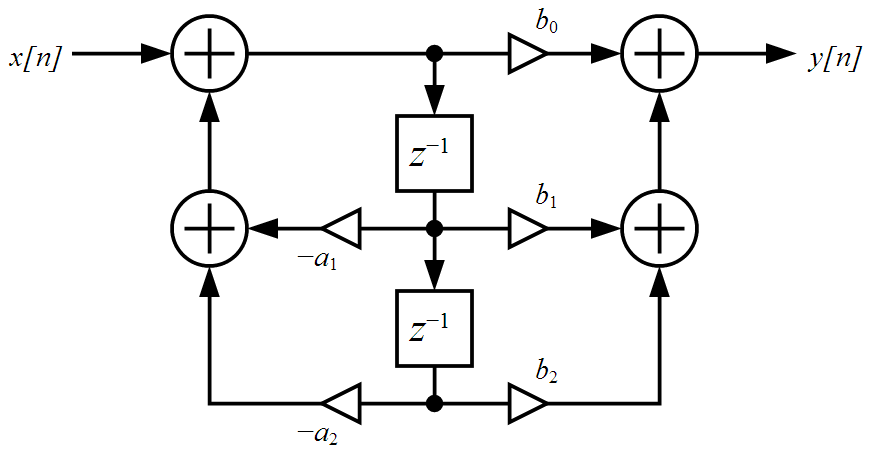
\includegraphics[width = 0.75\textwidth]{dfII.PNG}
	\end{center}
	\caption{Second order Direct Form II filter topology.}
	\label{fig:dfII}
\end{figure}

\begin{figure}[tbp]
	\begin{center}
		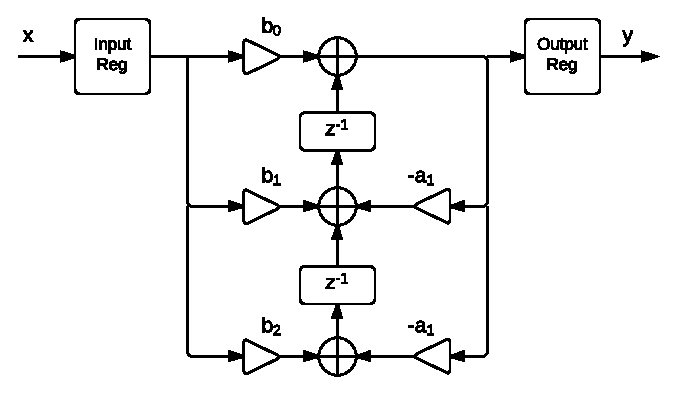
\includegraphics[width = 0.9\textwidth]{DirectFormIITransposed.pdf}
	\end{center}
	\caption{Second order Direct Form II Transposed filter topology.}
	\label{fig:df2t}
\end{figure}

As a second order IIR filter is settled upon, we need to chose what filter topology we will use. The candidates are Direct Forms I and II, and their transposed versions. It is immediately clear that the Direct Form II versions are better than the Direct Form I, as the number of state registers can be halved. Thus, the choice remains between regular and transposed version of Direct Form II.

In a software implementation, the difference between the two would be quite small, but in a hardware implementation they differ significantly. As can be seen in Figure~\ref{fig:dfII}, the Direct Form II filter topology requires an adder chain on the feedback path. This adder chain grows with one adder in the chain for every increased order of the filter.

Conversely, the Direct Form II Transposed filter topology only has a single 3-input adder for each stage, which is invariant to the filter order, as illustrated by Figure~\ref{fig:df2t}.
Thus, the critical path is constant for any order of the filter, and in all cases shorter than the non-transposed version. For these reasons, a Direct Form II Transposed filter topology is chosen. The timing of this filter is explored further in Section~\ref{sub:timing_analysis}.

% subsection filter_topology (end)

\begin{table}[tbp]
	\begin{center}
		\begin{lstlisting}
   FilterStructure: 'Direct-Form II Transposed, Second-Order Sections'
        Arithmetic: 'fixed'
         Numerator: [1 -1.979736328125 1]                  
       Denominator: [1 -1.97576904296875 0.996002197265625]
  PersistentMemory: false

   CoeffWordLength: 18                
     NumFracLength: 16                
     DenFracLength: 16
            Signed: true              
                                      
   InputWordLength: 16                
   InputFracLength: 0                 
                                      
  OutputWordLength: 16
  OutputFracLength: 0                 
                                      
   StateWordLength: 18
   StateFracLength: 2                 
                                      
 ProductWordLength: 36                
 NumProdFracLength: 16                
 DenProdFracLength: 16                
                                      
   AccumWordLength: 18                
NumAccumFracLength: 1                 
DenAccumFracLength: 1                 

         RoundMode: 'convergent'      
      OverflowMode: 'wrap'  
		\end{lstlisting}
	\end{center}
	\caption{Fixed point filter designed in MATLAB.}
	\label{tab:Hdsdsos}
\end{table}

\subsection{Quantization} % (fold)
\label{sub:quantization}

The effects of quantization depends entirely on the chosen filter topology. An FIR filter, which has no poles (except at the origin), can never become unstable, and as such, it is less sensitive to coefficient quantization. However, as seen in Section~\ref{sub:filter_design}, an FIR filter is simply not feasible for this application. Thus, as an IIR filter is required, careful consideration of the effects of quantization is required.

As this is a hardware implementation, it is possible to independently designate the bit widths for each of the different stages of the filter. That is, it is not only the bit width of the coefficients themselves that need to be tuned, but also the width of the data-paths, the input, the output, the state registers, the multipliers, and the adders. Furthermore, the resources of the target hardware architecture has to be considered.
For instance, the target FPGA has hardware multipliers that either multiply two 9 bit numbers, or alternatively, multiply two 18 bit numbers. That is, any bit-width between these two values would be underutilising the resources available on the FPGA.

During the initial design of the filter, it was established that a minimum of 12 bits was required for the coefficients of the filter in order to not create any resonance in the filter which would artificially amplify a portion of the passband.
Furthermore, it was empirically found that playback of the audio at 8 bits was simply not high enough fidelity to do the music justice. At 16 bits, the audio was deemed to be of good enough quality, and as such, the input and output widths of the filter are chosen to be 16 bits.

As we require at least 12 bits wide coefficients, and as the multipliers will have to be 18 bits wide, it is of penalty in terms of hardware resources to simply elect to have 18 bits wide coefficients. That is, as the multiplier blocks have dedicated input registers \cite{multipliers}, no extra registers are required to hold the coefficients.
Furthermore, as the coefficients are 18 bits, and the input is 16 bits, the rest of the system is required to be at least 16 bits wide in order to preserve the precision. However, as the adders and state stages are in series, it is in fact beneficial to have 2-3 more bits. Thus, it is elected to set the adder and state register bit-widths to 18 bits.

Finally, we must consider where to place the binary point in the fixed point representation. As this is a hardware implementation, shifts of the binary point are free. That is, we can independently assign the size of the fractional part of all the stages of the filter. 
In order to scale the binary point, we used the command \verb"Hdsdsos = autoscale(Hdsdsos, x)" from the digital filter toolbox in MATLAB.
This command will automatically scale the binary point of the different stages of the filter. It uses the provided input (in this case a 16 bit signed integer sample of the noisy music) to scale the binary point to include as much precision as possible while still avoiding overflow. The result of the operation can be seen in Figures~\ref{tab:Hdsdsos} and \ref{tab:fixedpoint_report}.

It should be noted that the aforementioned automatic scaling will optimise the filter for a representative input. Therefore, it will by design not guarantee the absence of overflow for any input. That is, if the filter were exposed to very extreme inputs, such as rail-to-rail amplitude signal, especially containing high amplitude 1kHz components, it would overflow.
To make a more robust filter, one could either over-estimate the range required during the binary-point placement, or implement saturating arithmetic. The trade-off is that the former will introduce more noise, while the latter will increase the critical path and use more hardware resources.

\begin{table}[tbp]
	\begin{center}
		\begin{lstlisting}
                               Fixed-Point Report                                          
            -------------------------------------------------------------------
                  Min       Max     |        Range       | Number of Overflows
            -------------------------------------------------------------------
      Input:      -32768      32767 |   -32768     32767 |   0/963144 (0%)
 Section In:      -32768      32767 |   -32768     32767 |  0/1926288 (0%)
Section Out:      -23436      23293 |  -131072    131071 |  0/1926288 (0%)
     Output:      -23436      23293 |   -32768     32767 |   0/963144 (0%)
     States:      -16423    16408.5 |   -32768  32767.75 |  0/1926288 (0%)
   Num Prod:   -64870.02      64872 |  -524288    524288 |  0/2889432 (0%)
   Den Prod:  -46021.588  46304.123 |  -524288    524288 |  0/1926288 (0%)
    Num Acc:      -64870      64872 |   -65536   65535.5 |  0/1926288 (0%)
    Den Acc:    -54472.5      54347 |   -65536   65535.5 |  0/1926288 (0%)
		\end{lstlisting}
	\end{center}
	\caption{Filtering Report generated when filtering the input sample}
	\label{tab:fixedpoint_report}
\end{table}

% subsection quantization (end)


\subsection{Filter Implementation} % (fold)
\label{sub:filter_implementation}

The filter described in Section~\ref{sub:quantization} is engineered to minimise quantisation noise while avoiding any overflow. This design is carried out using the digital filter toolbox in MATLAB.
This toolbox includes a feature for producing automatically generated Hardware Description Language (HDL).
Using the \verb"fdhdltool" command, we are able to generate Verilog HDL for the filter we have designed.
This tool provides us with a Verilog source file with the interface as shown in Figure~\ref{fig:Hdsdsos_interface}. The filter input and outputs are signed 16 bit integer representation with no fractional parts, as required.

As this method is guaranteed to generate the same digital filter that is already extensively tested in MATLAB, we are able to save a great deal of time in design and especially debugging of the filter core itself.
The time saved is put to use in performing the integration of the filter with the rest of the system, and especially in developing the custom memory controller described in Section~\ref{sub:hardware_implementation} and \ref{sub:tuning_for_speed}.

The HDL generation tool can also generate a second type of interface, one specifically designed to be capable of interfacing to a CPU for loading custom coefficients. However, due to the optimisations described in Section~\ref{sub:timing_analysis}, we elected to use hard-wired coefficients.
That is, the filter design tool cannot assume that the overall gain of the filter is unity when electing to supply coefficients from the processor interface.

However, it is possible to modify four (and with some modifications, five) out of the six coefficients while still maintaining the speed advantage. This design alteration is described in Section~\ref{sub:timing_analysis}. Unfortunately we did we did not have time to implement it.
As such, while the design is focused around having a fast system with variable coefficients, the system currently has hard-wired coefficients.

\begin{figure}[tbp]
	\begin{center}
		\begin{lstlisting}[language = Verilog]
module Hdsdsos_copy_hardwired
               (
                clk,
                clk_enable,
                reset,
                filter_in,
                filter_out
                );

input   clk; 
input   clk_enable; 
input   reset; 
input   signed [15:0] filter_in; //sfix16
output  signed [15:0] filter_out; //sfix16
		\end{lstlisting}
	\end{center}
	\caption{The interface of the automatically generated filter.}
	\label{fig:Hdsdsos_interface}
\end{figure}

% subsection filter_implementation (end)

\begin{landscape}
\begin{figure}[p]
	\begin{center}
		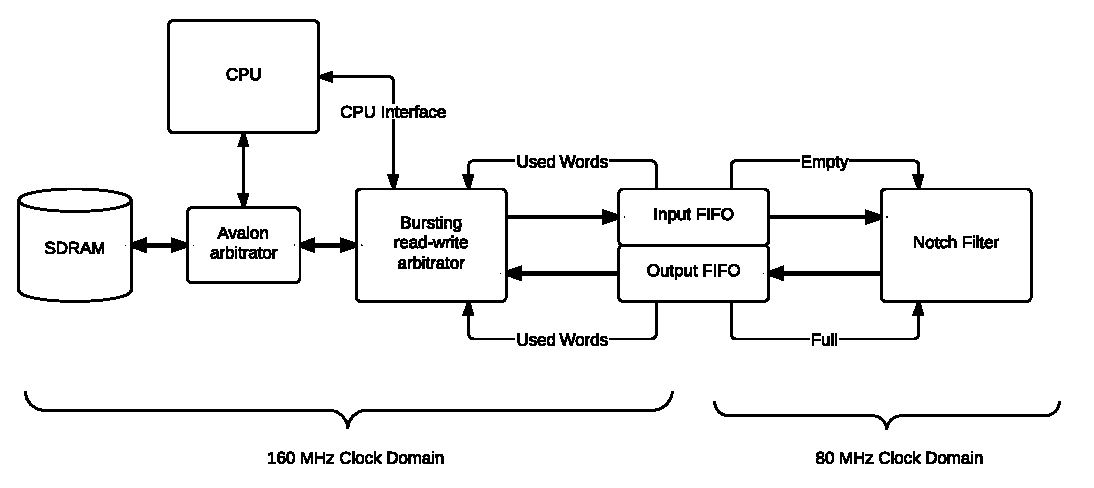
\includegraphics[width = 1.45\textwidth]{DSDNotch.pdf}
	\end{center}
	\caption{Block diagram of the Notch Filter hardware. FIFO buffers are used to allow efficient interleaved reads and writes to SDRAM. The buffers also serve as Clock Domain Crossing interfaces.}
	\label{fig:DSDNotch}
\end{figure}
\end{landscape}

\subsection{Hardware Implementation} % (fold)
\label{sub:hardware_implementation}

The filtering module, depicted in Figure~\ref{fig:DSDNotch}, is implemented as a memory mapped device. The CPU communicates with the hardware block by writing to an Avalon Memory-Mapped Slave interface.
The hardware module also has a Avalon Memory-Mapped Master interface so that the data required for the filtering operation can be fetched independently of the CPU, an operation known as Direct Memory Access (DMA).

The target architecture, the DE0 board, only has a single off chip memory with high memory bandwidth, the SDRAM memory. The Flash memory that is present on this board has such low memory bandwidth that if it were to be used, it would slow the system down several times over.
Thus, to complete the filtering operation, the data must be fetched from SDRAM, filtered, and then stored back in the same memory (but at a different location). The solution to this contention is to use a custom arbitrator that will interleave the reads and writes to SDRAM.

As non-sequential access to SDRAM is slow and sequential access is fast \cite{SDRAMDatasheet}, we use a feature of the Avalon interface known as Bursting \cite{AvalonSpec}. This feature locks the slave device, in this case the SDRAM controller, and forces it to fetch or store a sequential chunk of data as one uninterrupted operation.
That is, we are able to lock the arbitration of the Avalon interconnect to finish serving our sequential burst before it interleaves any requests from other masters, such as the CPU.

In order to maximise efficiency, we use a pair of First In First Out (FIFO) buffers to absorb the data that is obtained during a read burst, or to ensure sustained write throughput during a write burst.
These buffers are constructed from the architecture specific double ported memory blocks (M9K memory blocks) \cite{m9k}, as shown in Figure~\ref{fig:fifoblock}.
These FIFO blocks support different clocks on the read and write ports. Thus they can be, and are, used as Clock Domain Crossing (CDC) logic. This means that we can operate the filter core at a different clock speed than the rest of the system.

Another critical consideration is that once a burst has been initiated, it cannot be aborted \cite{AvalonSpec}.
Thus, the custom memory access controller will request at most the same number of words that remain unused in the input FIFO, as seen in Figure~\ref{fig:usedwords_burstcount}. The same thing applies to the write requests, the controller only requests to write as much data as is available in the output FIFO.
%TODO(figure of usedwords -> burstcount)

The core of the filter is limited to operating at 80MHz, while the rest of the system operates at 160MHz (see Section~\ref{sub:timing_analysis} for a detailed timing analysis). This means that even though the memory access is interleaved and cannot fetch one new word every clock cycle on average, the filter can still operate at almost full saturation.

While the Avalon Bus is a multi-mastered matrix \cite{AvalonSpec}, the heavily contended SDRAM is the bottle-neck for both the CPU and the filter hardware. For this reason we give the CPU both data and instruction caches, so that in the best case, it will not be completely starved during filtering.
However, in the worst case, as the Avalon arbitration is by default Round-Robin \cite{AvalonSpec}, the CPU will only be able to interleave with the filter hardware for a single word of data every 512 clock cycles.
This is deemed to not be a problem in this case, as the CPU performs no real-time critical tasks. If the CPU did require high priority access to the SDRAM in a different application, a priory aware arbitrator can be used.

\begin{figure}[bp]
	\begin{center}
		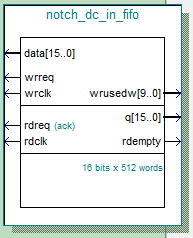
\includegraphics[width = 0.25\textwidth]{fifoBlock.PNG}
	\end{center}
	\caption{Block diagram of the First In First Out buffers used for both data buffering and Clock Domain Crossing.}
	\label{fig:fifoblock}
\end{figure}

\begin{figure}[p]
	\begin{center}
		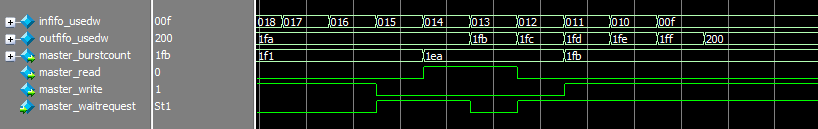
\includegraphics[width = \textwidth]{usedwords_burstcount.PNG}
	\end{center}
	\caption{Simulation of the system, showing how the number of requested words depends on how much free space/used words is present in the input/output FIFO. Note that there is a 2 cycle latency from the capture of the state of the FIFOs to the generation of the request. Also note that there is a long delay (30 cycles) after the read-request before any data is returned as the CPU is serviced in this period.}
	\label{fig:usedwords_burstcount}
\end{figure}

\begin{figure}[p]
	\begin{center}
		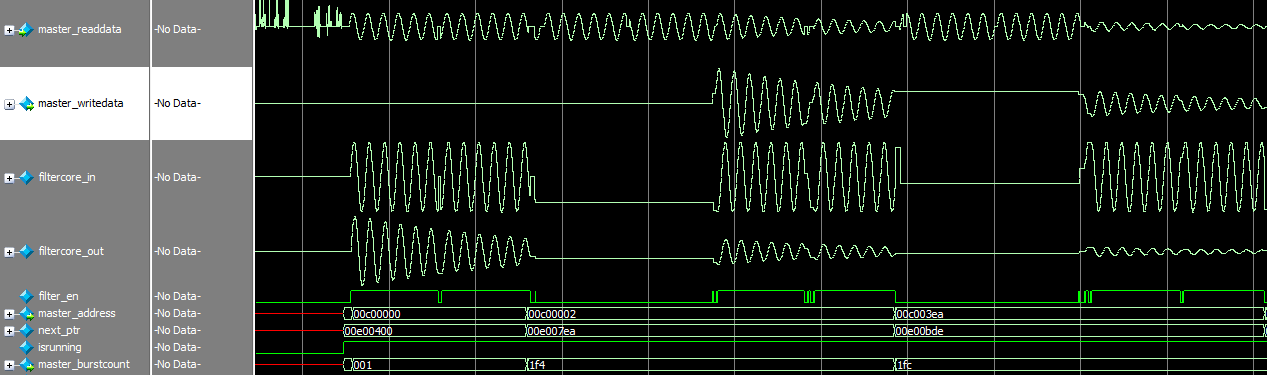
\includegraphics[width = \textwidth]{notchfilter_read_and_write_cropped.png}
	\end{center}
	\caption{Simulated interleaved operation of the filter. Note that both Clock Domains are simulated at 50MHz for clarity.}
	\label{fig:interleaved_sim}
\end{figure}

% subsection hardware_implementation (end)


\subsection{Timing analysis} % (fold)
\label{sub:timing_analysis}

\begin{figure}[tbp]
	\begin{center}
		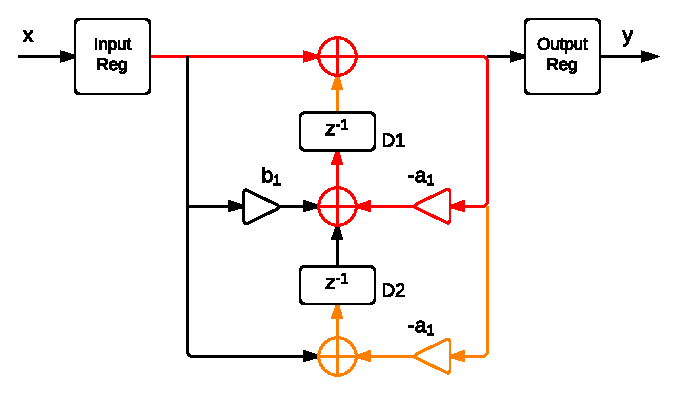
\includegraphics[width = 0.8\textwidth]{DirectFormIITransposedCritpath.pdf}
	\end{center}
	\caption{Annotated version of Figure~\ref{fig:df2t}, showing the main critical paths in the filter core. Shown in red is the critical path; from the input register to the delay register D1. Shown in orange are the alternative paths that have almost as little slack as the red path.}
	\label{fig:df2tCritpath}
\end{figure}

As mentioned in Section~\ref{sub:filter_topology}, Direct Form II Transposed is the chosen filter topology because of its superior timing characteristics. Nevertheless, the performance of the filter core is limited to processing 80 Million samples per second.
This is because the critical path, depicted in red in Figure~\ref{fig:df2tCritpath}, is forced to pass through two adder stages and one multiplier block.
Because the filter is recursive in nature, it is not possible to pipeline this path and as such it is not possible to increase the clock speed in a simple way. There is a method called Look-Ahead pipelining, which involves creating pole an zero pairs that cancel each other out, in order to be able to pipeline the feedback path.
However, this approach is deemed too involved for the purposes of this project.

One optimisation is however possible. As seen in Figure~\ref{fig:df2tCritpath}, the $b_0$ coefficient multiplier is not present. That is because, in our case, this coefficient, representing the overall gain of the system, is unity.
However, because of the linearity of IIR filters, if this gain is required to be non-unity, the multiplier can be moved to the other side of the input register.
Thus, the critical path is still maintained to be two adders and one multiplier for any Direct Form II Transposed filter implementation.
In our case, however, to optimise the resources used for the filter, we elected to optimise away both multiplier $b_0$ and $b_2$, as they are both unity for any notch filter.

Furthermore, when performing the timing analysis, we found that there are several paths that had a timing slack that is almost as tight as the critical path. These are depicted in orange in Figure~\ref{fig:df2tCritpath}.
That is, the paths from the input register to $D1$, from $D1$ to $D1$, from the input register to $D2$ and from $D1$ to $D2$, all have similar timing characteristics, and are the limiting paths in the design.

In fact, it is interesting to note that the high degree of similarity of the timing of these paths is expected. When inspecting the data-paths in a Direct Form II Transposed filter, as seen in Figure~\ref{fig:df2tCritpath}, all of these paths pass through two adders and one multiplier.
It is fascinating to see that the expected timing from a high level topology perspective translates so well to the final hardware implementation.

Moreover, as the FIFO buffers are used as Clock Domain Crossing interfaces, there is a risk of metastability. However as the generated clocks are phase locked, as they are generated using the same PLL module, this risk is minimal.
That is, as the clock frequency ratio is an exact integer, in this case two, the clock edges should always line up, and no metastability should be possible.
Nevertheless, the FIFO buffers are set-up to use two stage synchroniser stages to synchronise operation. While this may be overkill for the purposes of eliminating metastability, it does allow register re-timing to have more freedom to optimise the circuit for higher speed.

\begin{table}[tbp]
	\caption{Timing performance of the system at various operating conditions.}
	\label{tab:fmax}
	\begin{center}
		\begin{tabular}{l|cc}
		\hline

		\hline
			 										& $0^\circ$C 					& $85^\circ$C 	\\
		\hline
			\textbf{Maximum System Frequency} 		& 181.82 MHz					& 162.0 MHz 	\\
		\hline
			\textbf{Maximum Filter Core Frequency}	& 90.59 MHz						& 80.55 MHz 	\\
		\hline
			\textbf{Metastability MTBF}				& \textgreater 1 Billion Years	& \textgreater 1 Billion Years \\
		\hline

		\hline
		\end{tabular}
	\end{center}
\end{table}

% subsection timing_analysis (end)


\subsection{Tuning for Speed} % (fold)
\label{sub:tuning_for_speed}

As the target speed of the filtering module is quite high: 160MHz for the interface side, and 80MHz for the filtering side, some special considerations are required.
In particular, it was found that the address calculation for the fetch stage of the custom memory controller could not initially operate at 160MHz.
This was because, it was designed to update the current fetch pointer, compare it with the final pointer, and conditionally request new data. As these pointers are 32 bits wide, the critical path for this operation was simply too slow.

To remedy this, we redesigned the addressing to use a base pointer and an offset. This reduced the arithmetic to 20 bits. Furthermore, we pipelined the address calculation, so that a fetch operation has a latency of 2 cycles.
Thus, are were able meet the timing requirements for operation at the target clock frequency.

% subsection tuning_for_speed (end)


\subsection{Performance Results} % (fold)
\label{sub:performance_results}

The performance of the filter is benchmarked by executing a complete filtering pass of the filter, and observing a dedicated cycle-counting register. This register is simply reset at the start of the filtering operation and will increment every clock cycle until the filtering operation is complete.

Due to the efficiency of the custom bursting interleaved memory access controller, operating at twice the clock frequency of the filter core, as described in Section~\ref{sub:hardware_implementation}, we are able to exceed 90\% saturation of the filter core.
Thus, as the sampling rate of the data is 44.1 KHz, we are able to exceed 1600 times real-time performance.

\begin{table}[htbp]
	\caption{Performance results of the Notch Filter module.}
	\label{tab:notch_performance_results}
	\begin{center}
		\begin{tabular}{l|rl}
		\hline

		\hline
			\textbf{Time to process beeth5\_noise}	& 13.3 		& ms \\
		\hline
			\textbf{Length of beeth5\_noise}		& 963,144 	& Samples \\
		\hline
			\textbf{Average Throughput}				& 72.24 	& MSamples/s \\
		\hline
			\textbf{Filter Capacity}				& 80.0 		& MSamples/s \\
		\hline
			\textbf{Filter Saturation}				& 90.3 		& \% \\
		\hline
			%\textbf{Realtime Performance} 	& 1600		& Times faster than realtime \\
		%\hline

		\hline
		\end{tabular}
	\end{center}
\end{table}

% subsection performance_results (end)


\subsection{Resource Utilisation} % (fold)
\label{sub:resource_utilisation}

We chose to favour speed for this design as it makes for the most interesting optimisation trade-offs. That is, it is only when pressing for speed that one is required to think very hard about the critical path and the effects of pipe-lining.
Furthermore, as the device has more than 22 thousand logic elements, we found it was only natural to favour speed over area as the target device has a lot of spare resources.
That is, this filter module only consumes slightly over 5\% of the resources available in the device.

Outlined in Table~\ref{tab:resource_util_notch} is the resource utilisation per entity of the notch filter module.
The first thing to note is that we use a large number of logic cells and registers. This is primarily due to the fact that the synthesis optimisations are weighted towards speed.
Furthermore, register duplication, a physical synthesis optimisation, is enabled. That is, to enable register re-timing for high fanout signals, we allow for automatic generation of extra registers post-fanout.

An interesting note is that, as seen in Figure~\ref{fig:df2tCritpath}, we only require three multipliers. However, as the multipliers are arranged in pairs on this FPGA architecture, we end up using the next even number of multipliers, which in this case is four.

Also, we note that one way to cut down on the use of scarce resources, such as multiplier blocks, would be to use constant coefficient multipliers that are constructed out of adder trees. However, while there was not enough time to implement this interface, we intended the notch filter to accept new coefficients from the CPU.
Thus, to facilitate this feature, we are forced to use real multiplier blocks.

From a DSP perspective it is possible to use the Overlap-Save \cite{overlapsave} algorithm to combine the outputs of two IIR filter cores that execute on different segments of the input data in parallel.
However there would be no speed advantage in our case, as our implementation is already memory bandwidth limited with only one filter core, as seen in Table~\ref{tab:notch_performance_results}.

\begin{table}[tbp]
	\caption{Resource Utilisation of the Notch Filter module.}
	\label{tab:resource_util_notch}
	\begin{center}
		\begin{tabular}{l|ccc}
		\hline

		\hline
											& \textbf{Entire Module} 	& \textbf{Filter Core} 	& \textbf{Per FIFO}\\
		\hline
			\textbf{Logic Cells} 			& 1278 						& 322 					& 136 \\
		\hline
			\textbf{Dedicated Registers}	& 689						& 82 					& 117 \\
		\hline
			\textbf{M9K Memory Blocks}		& 2							& 0 					& 2 \\
		\hline
			\textbf{Multiplier Elements}	& 4							& 4 					& 0 \\
		\hline

		\hline
		\end{tabular}
	\end{center}
\end{table}

% subsection resource_utilisation (end)

\subsection{Operation} % (fold)
\label{sub:operation}

\begin{figure}[btp]
	\begin{center}
		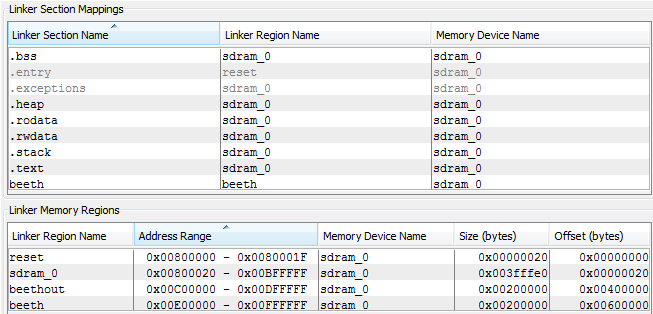
\includegraphics[width = \textwidth]{linkersections.PNG}
	\end{center}
	\caption{The linker sections and memory regions defined in the linker script.}
	\label{fig:linkersections}
\end{figure}

The audio data that will be filtered needs to be copied onto the SDRAM. We found that the easiest way to achieve this is to edit the linker script to reserve a memory region for the data. This is easily done using the Board Support Package Editor, as shown in Figure~\ref{fig:linkersections}.
Two megabytes is reserved for the input data, and another two megabytes for output data.

In order to get the 2MB data file onto the SDRAM, we define a linker section called \verb"beeth". We then generate a relocatable object file using the command line linker tool, and finally rename the automatically named data section to \verb"beeth".
The commands are as follows:

\begin{lstlisting}[frame=, aboveskip=3mm, belowskip=3mm]
nios2-elf-ld -r -b binary -o beeth.o beeth5_noise.bin
nios2-elf-objcopy --rename-section .data=beeth beeth.o beethsect.o
\end{lstlisting}

To link this object file to the rest of the system, we append the following to the end of the user-modifiable section of the Makefile:

\begin{lstlisting}[frame=, aboveskip=3mm, belowskip=3mm]
# User object files
OBJS := beethsect.o
\end{lstlisting}

As this object file is linked with the rest of the system, the following symbols are automatically defined:

\begin{lstlisting}[frame=, aboveskip=3mm, belowskip=3mm]
_binary_beeth5_noise_bin_start
_binary_beeth5_noise_bin_size
_binary_beeth5_noise_bin_end
\end{lstlisting}

This makes for seamless system integration, as these symbols can readily be used in the C code. Furthermore, the data itself will automatically be included in the .elf, and will as such automatically be downloaded to the target without requiring any extra user action.

We found that the easiest way to retrieve data from the system was to use the memory manipulation commands of GDB. That is, to download the memory contents to a file on the host machine, the following command is used in the GDB console:

\begin{lstlisting}[frame=, aboveskip=3mm, belowskip=3mm]
dump binary memory <file> <start_addr> <end_addr>
\end{lstlisting}

% subsection operation (end)

\subsection{Operational Results} % (fold)
\label{sub:operational_results}

We verify the operation of the hardware in both simulation and in hardware.
Shown in Figure~\ref{fig:notch_sim} are the simulation results of filtering during the first couple of microseconds of the operation of the filter.
This filter response matches the expected response, and also matches the response generated in hardware, as shown in Figure~\ref{fig:short_hardware_output}.
Shown in Figure~\ref{fig:notch_output} is the entire music sample after filtering. By a simple listening test, we also verify that no trace of the 1 kHz sine wave can be perceived, and no perceivable noise from the filtering operation is introduced.


\begin{figure}[p]
	\begin{center}
		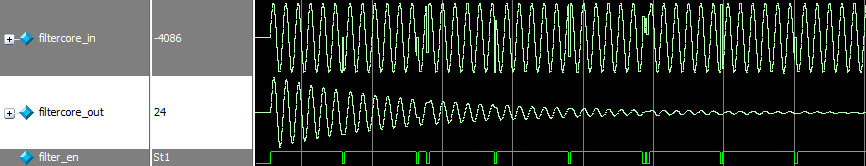
\includegraphics[width = \textwidth]{Notch_proper_data_cropped.png}
	\end{center}
	\caption{Simulation of filter in operation.}
	\label{fig:notch_sim}
\end{figure}

\begin{figure}[p]
	\begin{center}
		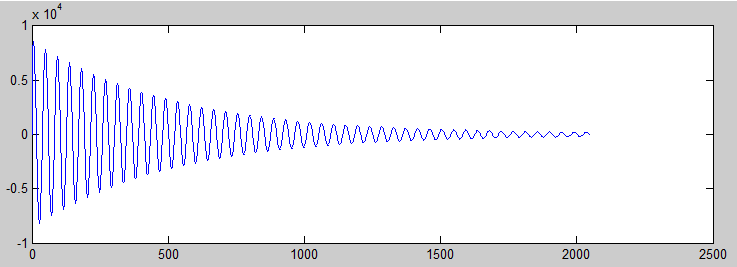
\includegraphics[width = \textwidth]{initaldatabackfromboard.PNG}
	\end{center}
	\caption{First 2048 output samples generated on hardware.}
	\label{fig:short_hardware_output}
\end{figure}

\begin{figure}[p]
	\begin{center}
		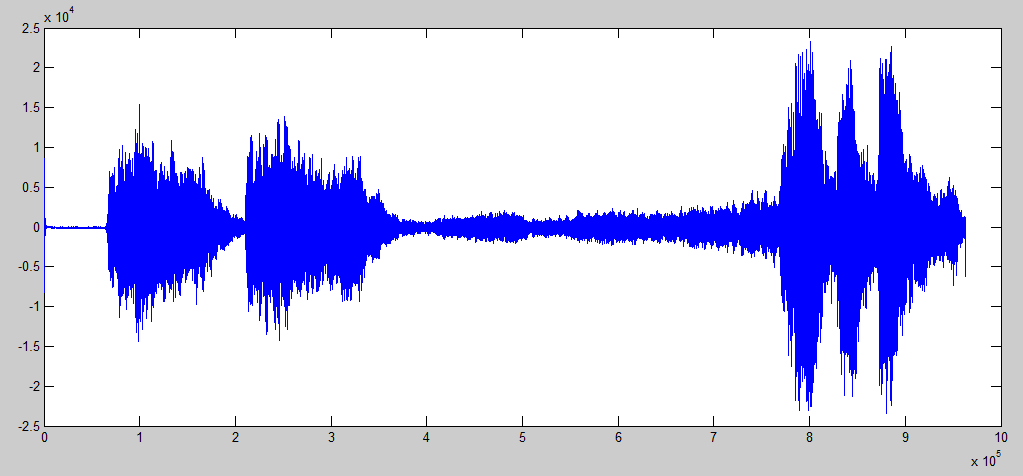
\includegraphics[width = \textwidth]{Notch_filtered_from_hardware.PNG}
	\end{center}
	\caption{Output after filtering on hardware.}
	\label{fig:notch_output}
\end{figure}

% subsection operational_results (end)

\subsection{Future Improvements} % (fold)
\label{sub:future_improvements}

The hardware was designed with the intention to be integrated with an interface to the CPU for updating filter coefficients. This was never implemented, so an obvious improvement would be to add this functionality.
As the multiplier blocks have input registers with enable lines on them \cite{multipliers}, it should be straightforward to memory map these registers to be accessible from the CPU interface.

We have designed a Pulse Width Modulation (PWM) audio output module. If implemented, this module would be able to accept 16 bit signed audio data through an Avalon Memory-Mapped Slave interface with only a single destination address.
As such, only a slight modification of the main filtering block would be required to be able to stream the output of the filter to this audio output module instead of writing the result back to the SDRAM.
The interface from the software's point of view would be the same, with the supplied destination address substituted for the PWM module's address.

% subsection future_improvements (end)

% section notch_filter (end)

\clearpage

\begin{thebibliography}{9}
	\bibitem{LUgen}
	Wei Zhang,
	\emph{Portable and Scalable FPGA-Based Acceleration of a Direct Linear System Solver}. \\
	\url{http://www.eecg.toronto.edu/~weizer/LUgen/WeiZhang.pdf}

	\bibitem{ieee754}
	IEEE,
	\emph{IEEE Standard for Floating-Point Arithmetic}. \\
	\url{http://ieeexplore.ieee.org/stampPDF/getPDF.jsp?tp=&arnumber=4610935}

	\bibitem{SDRAMDatasheet}
	Zentel Electronics Corp,
	\emph{64Mb Synchronous DRAM Specification}. \\
	\url{http://tsl-ds.googlecode.com/svn-history/r23/SDRAM/A3V64S40ETP_(Zentel).pdf}

	\bibitem{AvalonSpec}
	Altera Corp,
	\emph{Avalon Interface Specifications}. \\
	\url{http://www.altera.co.uk/literature/manual/mnl_avalon_spec.pdf}

	\bibitem{m9k}
	Altera Corp,
	\emph{Memory Blocks in the Cyclone III Device Family}. \\
	\url{http://www.altera.co.uk/literature/hb/cyc3/cyc3_ciii51004.pdf}

	\bibitem{multipliers}
	Altera Corp,
	\emph{Embedded Multipliers in the Cyclone III Device Family}. \\
	\url{http://www.altera.co.uk/literature/hb/cyc3/cyc3_ciii51005.pdf}

	%\bibitem{overlapsave}
	%Wikipedia,
	%\emph{Overlap–save method}. \\
	%\url{http://en.wikipedia.org/wiki/Overlap%E2%80%93save_method}

	\bibitem{overlapsave}
	Dr Patrick A Naylor,
	\emph{Digital Signal Processing Lecture Notes}. \\
	\url{https://bb.imperial.ac.uk/bbcswebdav/pid-84364-dt-content-rid-271372_1/courses/DSS-EE3_07-12_13/DSP3_Convolution.pdf}


\end{thebibliography}

\end{document}
